Exponential growth in generated raw data through various domains (e.g. security, bioinformatics, 
finance, etc.), has introduced new challenges to the research community for knowledge discovery 
and data analysis. The existing knowledge discovery and data engineering techniques have shown 
great success in many real-world applications, but the problem of learning from imbalanced data 
is a relatively new challenge. The problem is concerned with the performance of learning algorithms 
in the presence of underrepresented data and severe class distribution skews. Due to the 
characteristics of imbalanced data sets, learning from such data requires new principles, 
algorithms, and tools for knowledge discovery and information extraction. Though this section 
we will briefly go over the correspondent concepts and common approaches related to our study.

\subsection{Problem Definition}
Haibo He \cite{haibo_he_learning_2009}, defines imbalanced learning as “the learning process 
for data representation and information extraction with severe data distribution skews to develop 
effective decision boundaries to support the decision making process. The learning process could 
involve supervised, unsupervised, semi supervised learning or combination two or all of them.” 
In other words, it is learning from two (binary classification) or multiple classes (multi-class 
or multi-label classification) of data where the member classes have an unequal amount of examples.

Generally, any dataset with an unequal distribution of examples in between the member classes 
is technically imbalanced. But when a dataset is labeled as “imbalanced”, it means that through 
that dataset, there is a significant (or in some cases extreme) disproportion in between the number 
of examples of member classes.

In a binary classification problem with an imbalanced dataset, the class with lower number of 
instances is called the minority (positive) class and the one with the higher number of examples 
is called the majority (negative) class. In such a problem, Imbalance Ratio (IR) refers to the 
degree of existing imbalance in between the two member classes of the dataset \cite{orriols-puig_evolutionary_2009}. 
It is defined as the number of negative class examples divided by the number of positive class 
examples which is 10 for our example in Figure [\ref{fig:sampleBinaryImbalanced}]. In other words, 
IR 10 (or 1:10) refers to the fact that for every instance of the minority class, there exist 10 
instances in the majority class.  Figure [\ref{fig:sampleBinaryImbalanced}] shows a sample 
imbalanced dataset for a binary classification problem with an unequal distribution ratio of 1:10.

\begin{figure}[ht]
    \centering
    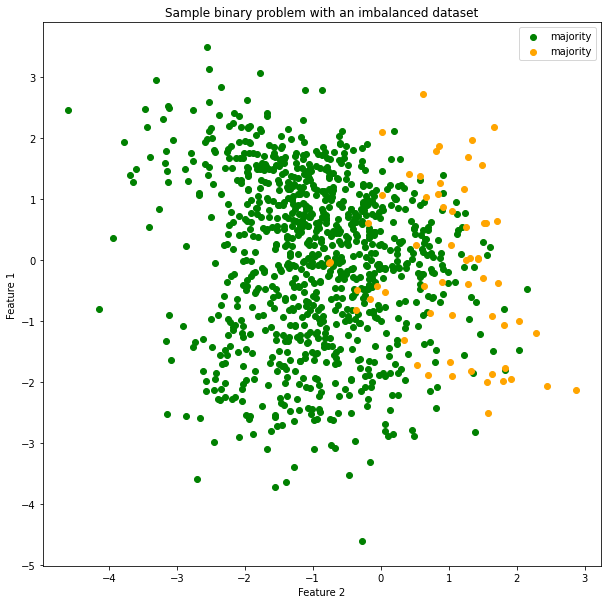
\includegraphics[width=0.60\textwidth]{figures/07SampleBinaryImbalanced.png}
    \caption{Sample binary imbalanced problem with ratio 1:10}
    \label{fig:sampleBinaryImbalanced}
\end{figure}

In bioinformatics (as we mentioned earlier through the last section) protein research is one of the 
fields where researchers try to identify the protein structures or its functions 
\cite{mishra_prediction_2014,lesh_complete_2003}. One of the popular approaches for solving 
these kinds of problems is protein classification. But the protein datasets are mostly imbalanced 
and therefore specific techniques are required. However, bioinformatics is not the only domain 
where researchers have to deal with imbalance datasets. Email classification \cite{bermejo_improving_2011}, 
face recognition \cite{yi-hung_liu_total_2005}, anomaly detection \cite{khreich_iterative_2010} and 
medical decision making \cite{mazurowski_training_2008} are among other applications where scientists 
need to learn and model on imbalanced sets of data.

Most of the imbalanced classification literature has been devoted to binary classification problems. 
However, there are also multi-class problems where the dataset is imbalanced 
\cite{mishra_prediction_2014,shuo_wang_multiclass_2012}. The approach for solving these sorts of 
problems normally includes transforming the multi-class classification problem into multi-binary 
classification problems. Which is one of the reasons the literature is mostly focused on binary 
classification problems. The multi-class and multi-label classification problem and approaches 
will be discussed in further details later through this section.

\subsection{Challenges in Imbalanced learning}
The main issue with the imbalanced problems is that normally, the underrepresented class 
(minority class instances) is the class of interest of the problem from the application point of 
view \cite{chawla_automatically_2008}. Usually, standard classifier learning algorithms are biased 
toward the majority class. 

In a standard learning algorithm, rules for prediction of the instances are positively weighted in 
favour of the accuracy metric or the corresponding cost function. In such an algorithm, specific 
rules for prediction of the examples from the minority class can be ignored (it treats them as noise), 
because more general rules are preferred. As a consequence, compared to instances from the majority 
class, minority class instances are more often misclassified. The amount of misclassified instances 
is even greater for highly imbalanced datasets.

By analyzing 26 binary-class datasets in a study, N. Japkowicz \cite{japkowicz_concept-learning_2001} 
shows how class imbalance impacts minority class classification performance. Figure 8 (being generated 
from the study) shows that the ratio between the minority and the majority class error rates is the 
greatest when the dataset is highly imbalanced. It also shows that the above error rate decreases as 
the amount of class imbalance decreases. With an error rate ratio above 1.0, it shows that class 
imbalance leads to a poorer performance on classifying minority class elements.

So, in similar problems, accuracy is no longer a proper metric for measuring the model performance 
in an imbalance scenario. Because it does not distinguish between the numbers of correctly classified 
examples of different classes. The accuracy only takes into account the total number of correctly 
classified instances. So, in an imbalance scenario, it often provides a high accuracy value with a 
very low true positive and a very high true negative value in the confusion matrix. We need to 
somehow construct classifiers that are biased toward the minority class, without being harmful 
to the accuracy over the majority class.

\begin{figure}[ht]
    \centering
    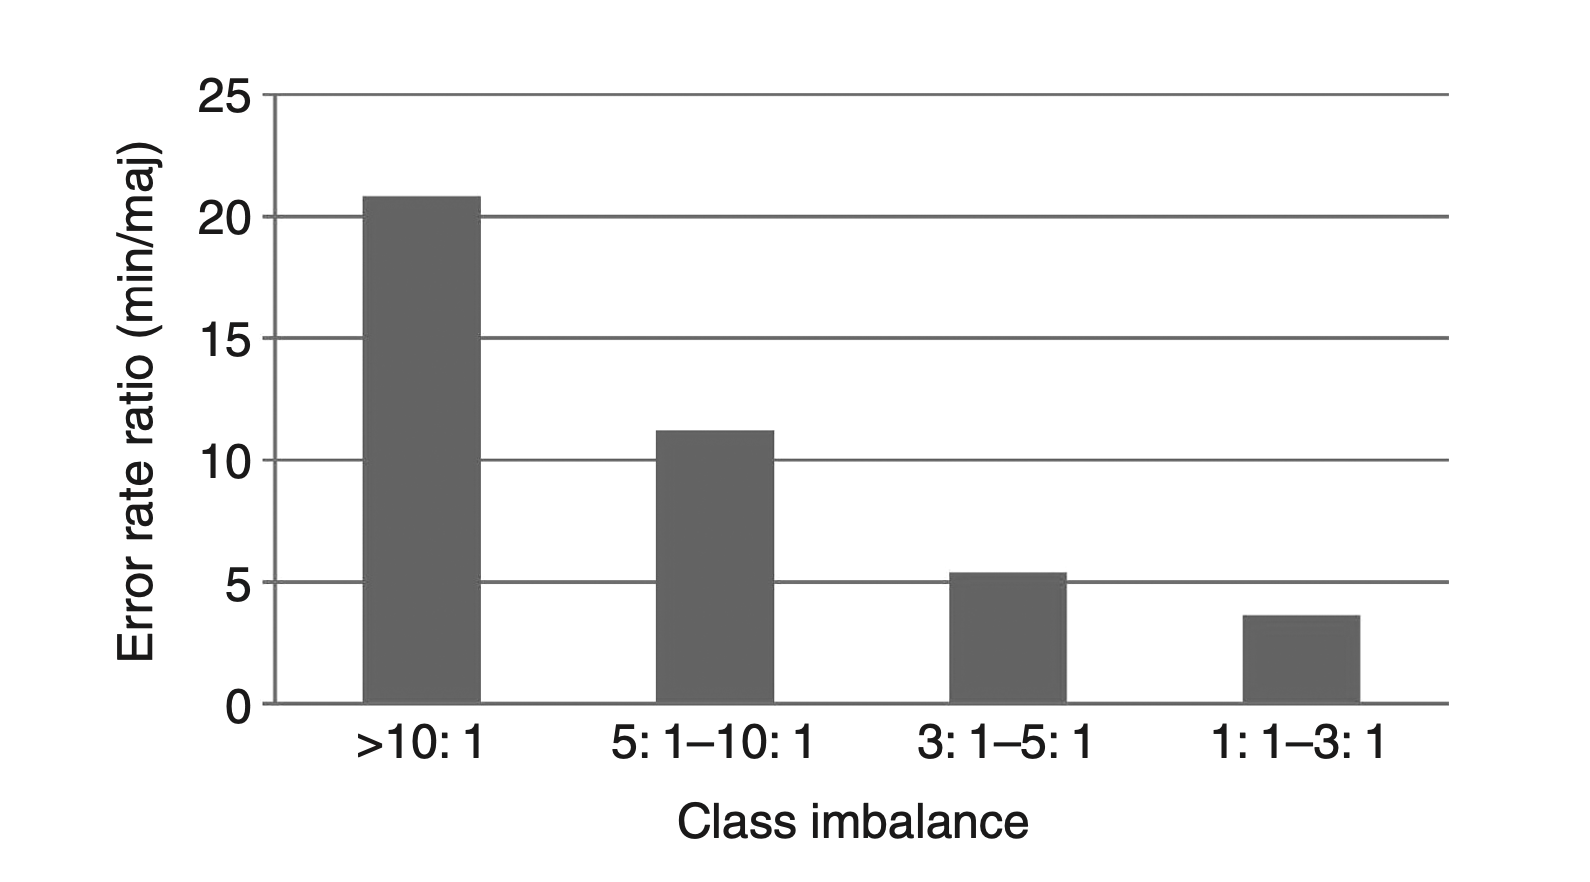
\includegraphics[width=0.60\textwidth]{figures/08errorRate.png}
    \caption{Impact of class imbalance on minority class performance \cite{japkowicz_concept-learning_2001}}
    \label{fig:errorRate}
\end{figure}

\textbf{Small sample size:} Generally imbalanced datasets have a lack of minority class examples. 
The ratio in between the minority and majority class examples indicates the degree of imbalance 
in a problem. Datasets with the higher degree of imbalance produce greater error rates.

\textbf{Overlapping (class separability):} When the elements from both minority and majority classes 
are mixed in the feature space, the decision boundary cannot be clearly established. As a result, 
more general rules will be applied to the problem in the classification phase, which will then lead 
to misclassifying some instances from the minority class \cite{garcia_k-nn_2008}.

\begin{figure}[ht]
    \centering
    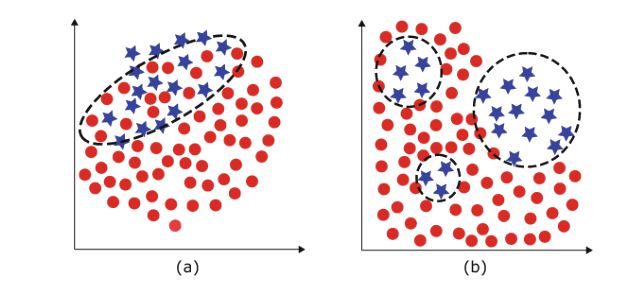
\includegraphics[width=0.60\textwidth]{figures/09overlapping.png}
    \caption{Imbalanced datasets difficulties (a) Class overlapping. (b) Small disjuncts \cite{fernandez_learning_2018}}
    \label{fig:overlapping}
\end{figure}

\textbf{Small disjuncts:} this problem occurs when the represented concept by the minority class is 
formed of subconcepts \cite{weiss_learning_2003}. As an example, in case of protein classification, the transporter 
proteins are classified into 7 substrate specific classes (amino acid transporter, anion 
transporter, cation transporter, electron transporter, protein/mRNA transporter, sugar transporter 
and other transporter). In most of the problems, small disjuncts increase the complexity of the 
problem because the amount of instances among them is not usually balanced.

\subsubsection{Imabalanced Classification Approaches}
Various techniques have been developed to correctly classify the minority class examples. 
These techniques can be categorized into four main groups, depending on the way they deal 
with the problem.

\textbf{Algorithm level} approaches are the ones trying to bias the existing learning 
algorithms towards the minority class \cite{lin_support_2002}. 
To achieve this goal, knowledge of both the corresponding classifier and the application 
domain is required to comprehend the reasons behind the classifier failure when the 
class distribution is uneven. 
 
\textbf{Data level} approaches are the ones trying to rebalance the class distribution 
by resampling the data space \cite{batista_study_2004,fernandez_study_2008}. 
This approach does not need to modify the learning algorithm since the effect caused 
by the imbalance will decrease after the rebalancing process.
 
\textbf{Cost-sensitive learning} approach falls between data and algorithm level 
approaches. In order to achieve the desired classification result on the minority 
class, It incorporates data level transformations and algorithm modifications 
\cite{ling_test_2006,chawla_automatically_2008}.
 
\textbf{Ensemble-based methods} are usually a combination of an ensemble learning 
algorithm and one of the approaches above \cite{galar_review_2012}. In the data level ensemble learning 
approach, the data will be preprocessed before training each classifier. On the 
other hand, the  cost-sensitive ensemble learning hybrid guides the cost minimization 
via the ensemble learning algorithm. 

\subsection{Performance Measurement}
The quality of the trained model is generally evaluated by analyzing how well it performs on the test data 
\cite{alsheikh-ali_public_2011}. To evaluate the model, the provided predictions of the trained classifier 
are compared to the true classes of test data and some performance measures will be then calculated. 
Depending on the provided information by the classifier, we can evaluate the model using either of following approaches:

\textbf{Nominal class} predictions where we compare the predicted class labels with the actual true class values, 
create a confusion matrix and then calculate the performance measure(s) for evaluating the model.

\textbf{Scoring Predictions} where we use the associated scores (or the probability values) of the predictions 
to grade test examples according to the likelihood of pertaining to a class and then calculate the required 
measure for evaluating the model.

For the \textbf{nominal class predictions}, a convenient way for summarizing the performance of classifiers 
is to create a confusion matrix [\ref{fig:confusionMatrix}]. The columns of the confusion matrix represent the counts of instances in 
the predicted classes while the rows represent the counts of instances in the actual classes (or vice versa). 
In this matrix (for a binary class problem), TP and TN (for true positives /true negatives ) indicate the 
correct classification of positive and negative instances, respectively, and FN and FP 
(for false negatives /false positives ) indicate positive/negative instances misclassified as 
negative/positive, respectively. 

\begin{figure}[ht]
    \centering
    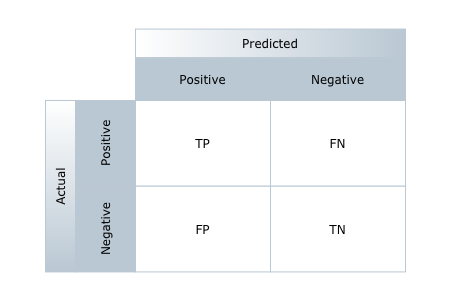
\includegraphics[width=0.60\textwidth]{figures/10ConfusionMatrix.png}
    \caption{Confusion Matrix}
    \label{fig:confusionMatrix}
\end{figure}

Various performance measures could be calculated using the confusion matrix. These measures correspond 
to different views of what constitutes a good classifier. Using these different measures we can summarize 
the confusion matrix into performance metrics so that we can assess the strengths and weaknesses of a 
classifier from different perspectives.

The first and mostly used measure for evaluating the classification performance is accuracy. 
Accuracy [\ref{eq:accuracy}] is the ratio of the correctly classified instances to the total instances of 
the test set. In the confusion matrix, it is the sum of the true positive and the true negative 
(which in the binary case is TP + TN) divided by the total number of instances. Error rate [\ref{eq:errorRate}] 
is the percentage of incorrectly classified instances.

\begin{equation}
    Accuracy = \frac{TP+TN}{N} 
    \label{eq:accuracy}
\end{equation}

\begin{equation}
    Error = 1-Accuracy = \frac{FP+FN}{N} 
    \label{eq:errorRate}
\end{equation}

The accuracy / error rate is widely used as a performance measure in various problems. 
But it is not a proper measure in the imbalance scenario [26]. In a highly imbalanced 
scenario, It is easy to obtain high accuracy \ref{fig:confusionMatrixSameAccuracy}. 
It also assumes that errors have an equal cost. But, in the imbalanced classification 
problem, when compared to the instance of the majority class, misclassifying instances 
of the minority class is much costlier.

\begin{figure}[ht]
    \centering
    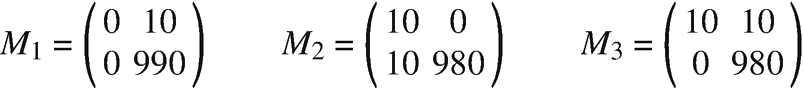
\includegraphics[width=0.60\textwidth]{figures/11ConfusionSameAccuracy.png}
    \caption{3 confusion matrices with the same accuracy}
    \label{fig:confusionMatrixSameAccuracy}
\end{figure}

Due to the drawbacks of the accuracy for assessing the performance of the models in an 
imbalanced scenario, we need some other measures along with the accuracy through which 
we could obtain more insight on the performance of the model. There are various measures 
such as Kappa, G-mean, G-measure, Sensitivity, Specificity, MCC, Precision, Recall, 
F-Measure etc. that could be calculated from the confusion matrix, but the common ones 
for the problems with an imbalance datasets are as follow:

\subsubsection{Sensitivity and Specificity:}

The sensitivity of a classifier [\ref{eq:sensitivity}] corresponds to its true positive rate (TPR). 
It is the proportion of the positive examples being predicted as positive by the model. 
The complementary metric to the sensitivity is called the specificity of the classifier 
[\ref{eq:specificity}]. It corresponds to the proportion of negative examples that are being 
predicted correctly. These two metrics are typically used to assess the effectiveness of 
a clinical test in detecting a disease.

\begin{equation}
    Sensitivity = \frac{TP}{TP+FN} 
    \label{eq:sensitivity}
\end{equation}

\begin{equation}
    Specificity = \frac{TN}{TN+FP} 
    \label{eq:specificity}
\end{equation}

\subsubsection{MCC}
The MCC \cite{matthews1975comparison} is a measure that comes from the field of Bioinformatics, 
where class imbalance occurs very often [\ref{eq:mcc}]. It is a measure that takes into account 
all values of the confusion matrix, considering errors and correct classification in both classes. 
MCC ranges from 1 (when the classification is always wrong) to 0 (when it is no better than random) 
to 1 (when it is always correct).

\begin{equation}
    MCC = \frac{(TP*TN)-(FP*FN)}{\sqrt(TP+FP)(TP+FN)(TN+FP)(TN+FN)} 
    \label{eq:mcc}
\end{equation}

\subsubsection{Precision and Recall}

The precision of a classifier indicates how precise the model is when identifying the examples 
of a given class [\ref{eq:precision}]. It assesses whether the proportion of the examples being predicted 
as positive are truly positive or not. In this pair, recall is the same as the Sensitivity measure 
being mentioned above [\ref{eq:recall}]. These two measures are commonly used together where scientists 
are interested in the proportion of the identified relevant information along with the amount of 
actually relevant information.

\begin{equation}
    Precision = \frac{TP}{TP+FP} 
    \label{eq:precision}
\end{equation}
\begin{equation}
    Recall = \frac{TP}{TP+FN} 
    \label{eq:recall}
\end{equation}

\subsubsection{Geometric Mean}
Introduced by Kubat et al. \cite{kubat1998machine}, The G-mean [\ref{eq:gmean}] was a response to the class 
imbalance problem in an effort to create a single metric by combining a pair. This measure takes 
into account the relative balance of the classifier’s performance on both the positive and the 
negative classes. By defining a function which takes into account both the sensitivity and the 
specificity of the classifier.

\begin{equation}
    G-Mean = \sqrt(Sensitivity*Specificity) 
    \label{eq:gmean}
\end{equation}

\subsubsection{F-Measure}
The F-measure is a combination metric whose purpose is to combine the values of the precision and 
recall of a classifier to a single scalar [\ref{eq:fmeasure}]. It does so in a different way than the G-mean, 
as it allows the user to weigh the contribution of each component as desired.

\begin{equation}
    F \alpha = \frac{(1+\alpha)[Precision*Recall]}{[\alpha*Precision]+Recall} 
    \label{eq:fmeasure}
\end{equation}

\subsubsection{Scoring Predictions}

Let’s consider a classifier that gives a numeric score or a probability of an instance belonging to a 
class. Therefore, instead of a simple positive or negative prediction, we will have a score 
(probability value) for each predicted instance. instances with higher probabilities are more 
likely to have to be classified as positive.

Having a probability value (or a score) for an instance, gives us more control over the results. 
We can determine our own threshold to interpret the result of the classifier. Different thresholds 
will result in different values for the confusion matrix elements (TP, TN, FP, FN) which leads to 
different values for the calculated measures (e.g sensitivity, specificity, etc.).

A higher threshold will reduce the false positive rate (FPR) and increase the false negative rate 
(FNR), because less instances will be classified as positive. On the other hand, a lower threshold 
will increase the FPR and reduce the FNR value. To evaluate these kinds of models, we use the ROC curve.

The ROC curve \cite{fawcett2006introduction} is a graphical evaluation method that is not dependent 
on a specific threshold. A ROC graph is a plot of False Positive Rate (FPR) on the x-axis, and 
True Positive Rate (TPR) on the y-axis. The threshold starts with the one that produces the highest 
score, all the way to the lowest score. For each possible value of the threshold, there is a point 
in the ROC space based on the values of FPR and TPR for that threshold.

The AUC (or the Area Under Curve) of the ROC can be interpreted as the probability that the 
probabilities (or scores) given by a classifier will rank a randomly chosen positive instance 
higher than a randomly chosen negative one. The AUC ROC of random guessing is 0.5, so it is 
expected that the AUC ROC for a useful classifier is higher than 0.5 and the ideal classifier 
would produce an AUC ROC value of 1.

\begin{figure}[ht]
    \centering
    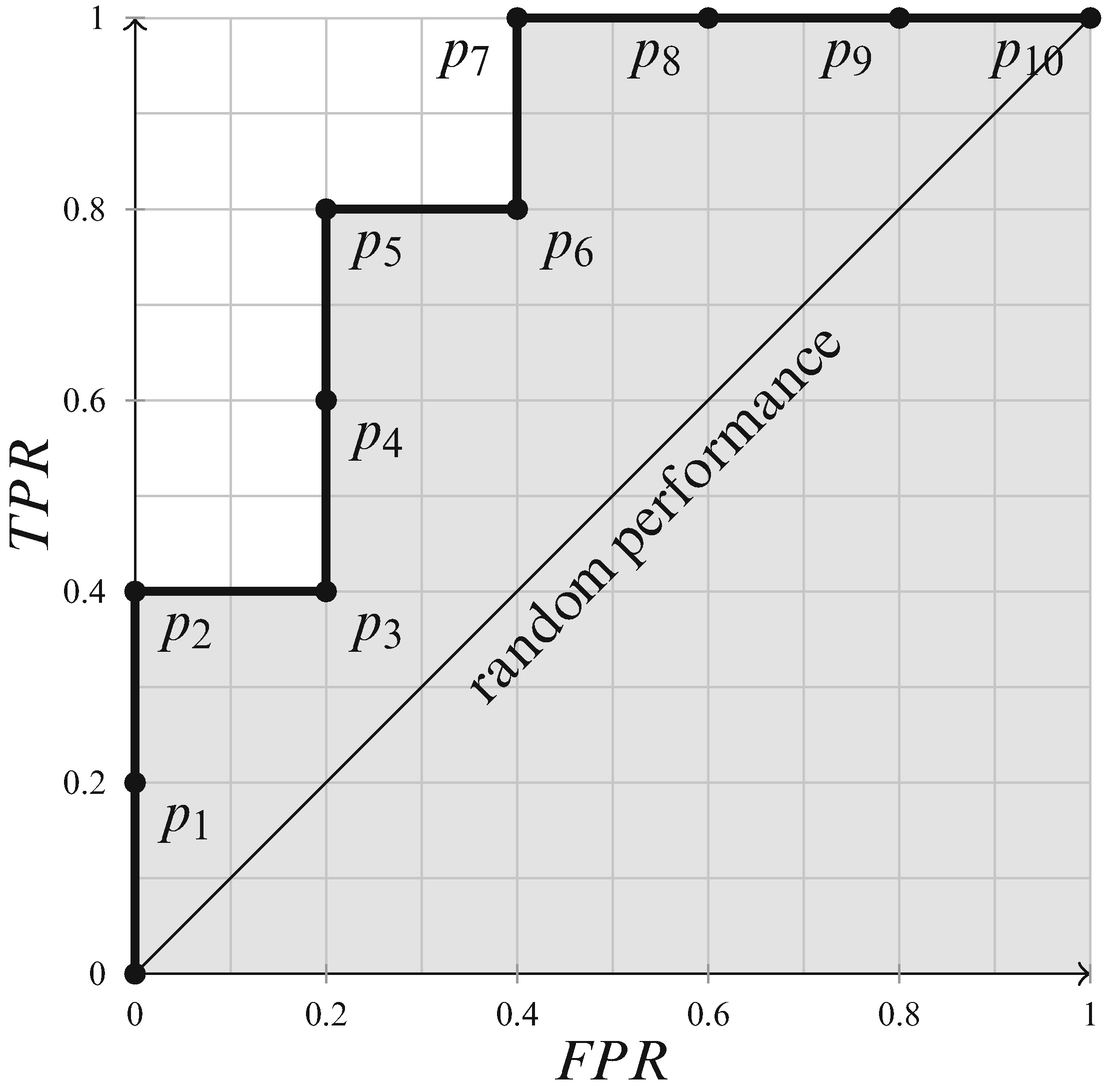
\includegraphics[width=0.60\textwidth]{figures/12RocExample.png}
    \caption{Sample ROC graph}
    \label{fig:roc}
\end{figure}


\subsection{Dealing with multiple classes}

Traditionally, when we talk about imbalance classification, we refer to a binary classification 
problem with one class having more instances (majority) than the other one (minority)
\cite{haibo_he_learning_2009, branco2015survey}. However, there are many cases in real life 
that we have to deal with more than two classes. Target detection \cite{razakarivony2016vehicle},  
microarray research \cite{yu2013recognition} and protein classification \cite{zhao2008protein} 
are among those topics where we face multiple classes of data and the distribution of examples among 
the classes is not homogeneous.
 
In such cases, the problem that must be taken into account is the presence of multi-minority 
and multi-majority classes \cite{wang2016dealing} which somehow implies that we can no 
longer just focus on a single class to reinforce the learning models towards it. Also, 
any further complication (e.g. overlapping classes) can affect the problem severely and must be 
analyzed in depth \cite{saez2016analyzing}.

To address all the issues, a simple and effective way is to somehow decompose the multi-class 
imbalance problem into multiple binary-class problems with an imbalanced dataset. We can 
then assign a classifier to each decomposed problem and the outputs of all the classifiers 
for a given instance will be aggregated to make the final decision \cite{kuncheva2014combining}. 
Therefore, the difficulty in addressing the multi-class problem will be shifted from the classifier 
itself to the combination stage. 

The underlying idea is to undertake the multi-classification using binary classifiers 
with a divide and conquer strategy. Among decomposition strategies, the most popular 
techniques are the One-vs-One (OVO) \cite{hastie1998classification,knerr1990single}
and One-vs-All (OVA) \cite{clark1991rule,anand1995efficient}.

\subsubsection{The One-vs-All Scheme (OVA)}
In OVA decomposition strategy, a problem with $n$ classes of instances is divided into $n$ 
binary problems. An independent classifier will be then assigned to each binary sub-problem which 
is responsible for distinguishing one of the classes from all other classes. The learning 
step of the classifiers is done using the whole training data, considering the patterns from 
the single class as positives and all other examples as negatives. \ref{fig:ova} shows the OVA 
binarization technique for a 3-class problem.

\begin{figure}[ht]
    \centering
    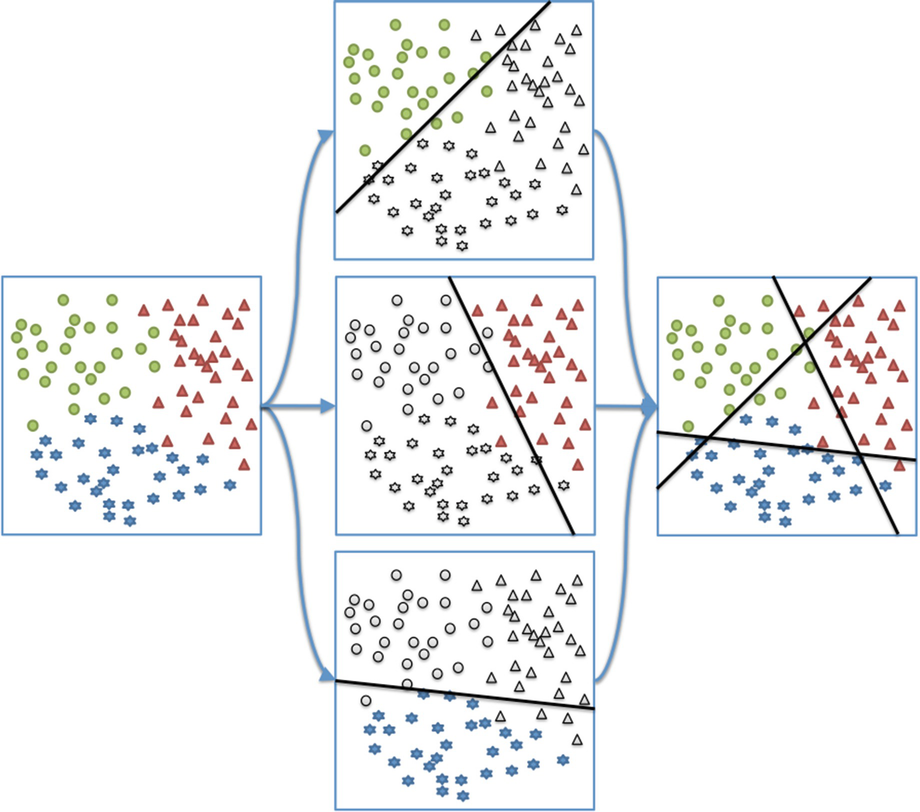
\includegraphics[width=0.60\textwidth]{figures/11ova.png}
    \caption{Sample OVA binarization technique for a 3-class problem \cite{fernandez_learning_2018}}
    \label{fig:ova}
\end{figure}

\subsubsection{The One-vs-One Scheme (OVO)}
In this strategy, a problem with $n$ classes is divided into $n*(n+1)/2$  binary class 
problems (one for each possible pair of classes). An independent classifier will be then 
assigned to each binary sub-problem. For each binary subset, the learning phase is then 
carried out using a subset of the original training instances with only those that contain 
any of the two classes. And the instances with different class labels are simply ignored. 
\ref{fig:ovo} shows the OVO binarization technique for a 3-class problem.

\begin{figure}[ht]
    \centering
    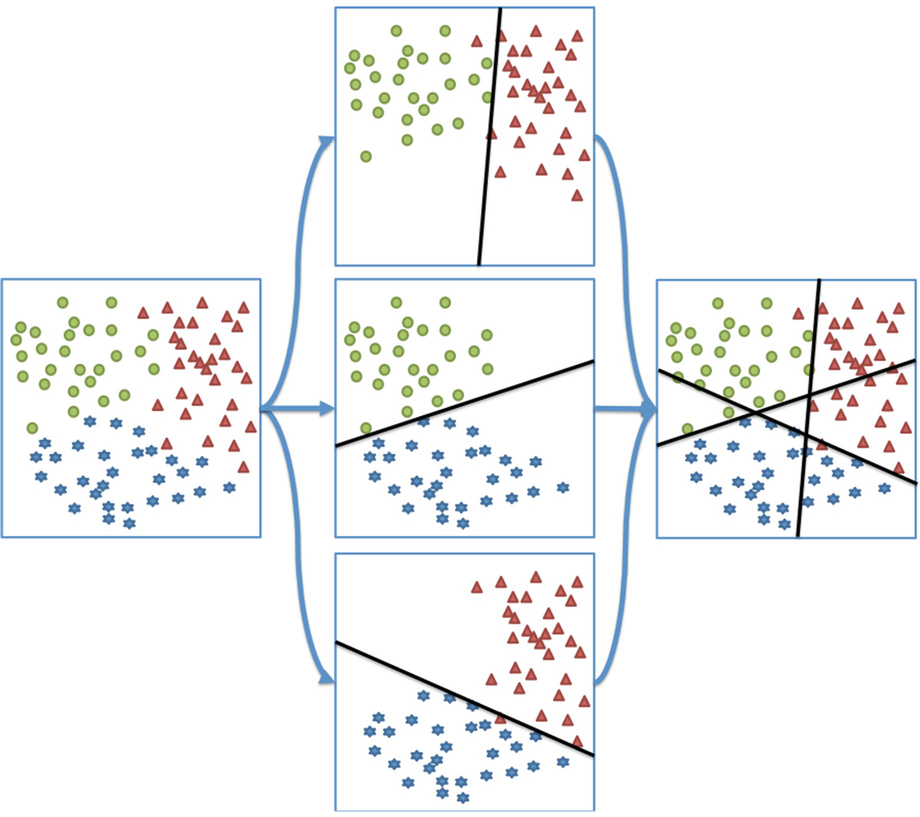
\includegraphics[width=0.60\textwidth]{figures/12ovo.png}
    \caption{Sample OVO binarization technique for a 3-class problem \cite{fernandez_learning_2018}}
    \label{fig:ovo}
\end{figure}

\subsubsection{Multi-class Classification vs Multi Label Classification}
Multi-class classification refers to a classification task with more than two classes. The 
classification makes the assumption that one and only one label will be assigned to an instance  
through the prediction phase. As an example we can consider a fruit image classification problem 
with 3 classes of Orange, Apple and Tangerine. Using a multi-class classification approach, 
through the prediction phase, an image can be either an apple or an orange or a tangerine.
 
Multi-label (multi-output) classification on the other hand, is a generalization of multiclass 
classification where multiple labels may be assigned to each instance. As an example, we can 
consider a comment classification problem with 4 classes of Positive, Negative, Toxic, Insulting. 
Using a multi-label classification approach, an instance can be both Negative and Toxic. 
While another one can be just Negative.

\subsubsection{Aggregation}
After decomposing the initial multi-class problem into multiple binary class problems, a classifier 
will be assigned to each problem. As an example, in an OVA case, a problem with 3 classes 
(labeled as Orange, Tangerine and Apple) will be decomposed into a 3 binary class problem with its 
own classifier.  In order to classify a new example, the instance will be submitted to all the 
classifiers. Then, the predictions of all the classifiers are considered in the combination phase, 
which is also known as classifier fusion or aggregation \cite{wozniak2014survey}.

In case of Multi-class classification problems, since we are looking for one and only one prediction 
for each instance, in the aggregation phase, the result with the highest score/probability will 
be chosen as the final prediction for that instance. In the example mentioned above,  if 
classifier 1 predicts Orange with 0.75, classifier 2 predicts not a Tangerine with 0.64 and 
classifier 3 predicts Apple with 0.82, then the final predicted label will be an Apple. The 
predicted results are then put together and compared to the actual labels to generate the 
confusion matrix which is then used to calculate the performance matrix.

In case of Multi-label classification problems, since all the labels are acceptable, then all 
will be considered. As an example, in a comment classification problem, a comment can be both 
Negative and an Insult. 


\subsubsection{Threshold-Moving}
Many machine learning algorithms are capable of producing a probability or a score value for 
an instance of a dataset. This value needs to be interpreted before being mapped to a class 
label. The decision for converting a predicted probability or scoring into a class label is 
governed by a parameter referred to as the “decision threshold,” “discrimination threshold,” 
or simply the “threshold.” The default value for the threshold is 0.5 for normalized predicted 
probabilities or scores in the range between 0 or 1.

When studying problems with imbalanced data, using the classifiers produced by standard 
machine learning algorithms without adjusting the output threshold may well be a critical 
mistake” \cite{provost_machine_2000}. So, for those classification problems with an 
imbalance dataset, the default threshold can result in poor performance. A simple and 
straightforward approach for improving the performance of a classifier that predicts and 
produces probability values for instances of an imbalanced classification problem, is 
tuning the default threshold being used by the algorithm for mapping the probability 
values to class labels.

In a problem, if a specific threshold is considered, the threshold should be applied to each 
classifier before the aggregation phase. For example in the case of the classifier for Oranges, 
Tangerines and Apples, if the considered threshold is 0.71 (which means the scores/probabilities 
above that threshold is considered as positive) then the results will be Oranges (classifier 1), 
not a Tangerine (classifier 2) and not an Apple (Classifier 3). Which then leads to the final 
prediction of the Orange as the label for the instance after aggregation. The threshold-moving 
effect could be observed and analyzed through the ROC/AUC  or Precision/Recall curves.

\subsubsection{Micro averaging vs Macro averaging}
Considering a performance metric $P$ being calculated based on the confusion matrix elements 
(true positives ($tp$), true negatives ($tn$), false positives ($fp$),false negatives ($fn$). 
The macro and micro averages of a specific measure can be calculated as follow:

\begin{equation}
    P_{macro} = \frac{1}{q} \sum_{q}^{\lambda =1} P(tp_{\lambda},tn_{\lambda},fp_{\lambda},fn_{\lambda})
    \label{eq:macro}
\end{equation}

\begin{equation}
    P_{macro} = P (\sum_{q}^{\lambda =1}tp_{\lambda}, \sum_{q}^{\lambda =1}tn_{\lambda}, \sum_{q}^{\lambda =1}fp_{\lambda}, \sum_{q}^{\lambda =1}tp_{\lambda})
    \label{eq:micro}
\end{equation}
Where $\lambda$ is a Label and $L = {\lambda_{j}: j= 1...q}$ is the set of all labels.

For a problem in machine learning, normally, we take different samples from a dataset and then 
we run the model on all of those samples independently to estimate the skill of a machine learning 
model on the unseen data. A popular technique in this area is k-fold cross validation 
\cite{james_introduction_2013}. In order to produce the final metrics for a model, we need 
to average in between a performance metric (e.g. sensitivity) of different classifiers in 
a model or multiple models on different samples of data (which is the case in multi-class 
or multi-label classification problems). The averaging could be done by either macro or 
micro averaging approach which can produce different results.

Micro and macro-averages compute slightly different things. So, their generated result's interpretation is 
different from one another. Macro-average approach, computes the metric independently for each class 
and then takes the average (hence treating all classes equally), whereas the micro-average approach, 
aggregates the contributions of all classes to compute the average metric \cite{sokolova_systematic_2009}. 
For imbalanced problems involving multiple classes, the micro-averaging approach is preferable.


\subsubsection{Support Vector Machine (SVM)}
Algorithm-level solutions concentrate on modifying existing learners methods for handling 
imbalanced datasets. Instead of focusing on modifying the training set in order to combat 
class skew, this approach aims at modifying the classifier learning procedure itself to 
alleviate their bias towards majority class instead on altering the supplied 
training set \cite{krawczyk2016learning}.

Due to their powerful generalization abilities, convergent properties and flexibility in 
adapting to various learning difficulties, Support Vector Machines (SVMs)\cite{vapnik2013nature} 
are among the most popular algorithms for pattern classification in this category. 
The algorithm is effective in high dimensional spaces and it accepts different Kernel 
functions for the decision making process.

\begin{figure}[ht]
    \centering
    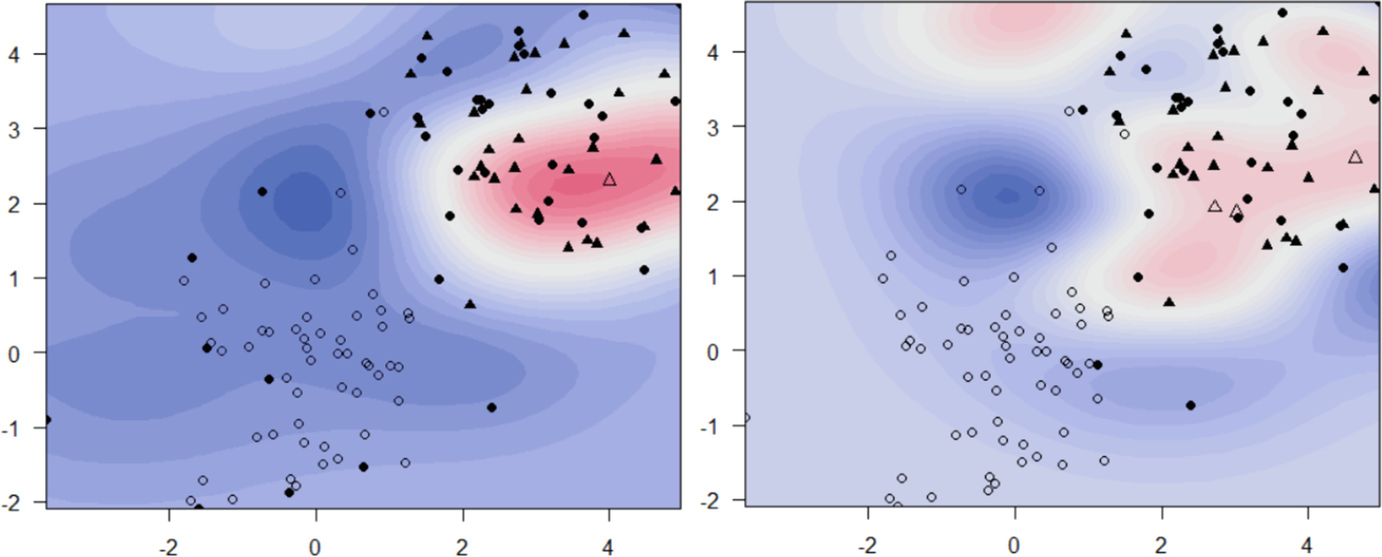
\includegraphics[width=0.60\textwidth]{figures/13svmAlgorithm.png}
    \caption{Support Vector Machine boundries for an imbalanced dataset: 
    (left) standard approach; (right) instance-level 
    weighting \cite{fernandez_learning_2018}}
    \label{fig:svmBoundries}
\end{figure}

Fernandez et al \cite{fernandez_learning_2018} explains the support vector machine, involved parameters 
and the algorithm's related imbalanced classification concerns as:

SVM algorithm aims at finding the optimal hyperplane which separates instances into two 
classes. Traditional linear classifiers offer many desirable properties, but they are not 
able to cope with complex data structures. SVM transforms the input instances into a higher 
dimensional artificial feature space(s). So, by using a non-linear mapping $\theta$, 
it can achieve a linear separation between classes in the new space, 
which in turn translates to a non-linear decision boundary in the original feature space. 
The potential separating hyperplane can be represented as:

\begin{equation}
    w.\theta(x)+b=0
    \label{eq:svmBasic}
\end{equation}
Where $w$ stands for a weight vector normal to this hyperplane. In case of considered data 
are linearly separable, the decision hyperplane characterized by a maximum margin can be 
obtained by optimization of margin as: $ min(1/2 w.w) $ subject to 
$\forall_{i=1...l}, y_{i}(w.\theta(x_{i})+b)\geq 1$ where $l$ stands for the number of training instances.

However, datasets are rarely linearly separable. So, we need to modify the 
the equation to include the possibilities of classifying some of training instances, 
to achieve greater generalization and reduce overfitting. This is 
done by using slack variable associated with $i-th$ instance $\epsilon_{i} \geq 0$. 
This allows to rewrite the margin optimization problem as soft margin:

\begin{equation}
    min(\frac{1}{2}w.w+C\sum_{i=1}^{l}\epsilon_{i}) \\
    \label{eq:svmSoftMargin}
\end{equation}
Subject to $\forall_{i=1...l}, \forall_{\epsilon\geq0}, y_{i}(w.\theta(x_{i})+b)\geq 1-\epsilon_{i}$
Where $C$ stands for the regularization parameter that controls the trade-off between maximizing 
the separation margin between classes and minimizing the number of misclassified instances.
This is a quadratic optimization problem that can be solved by transforming it into 
Lagrangian optimization problem with the following dual form:

\begin{equation}
    max_{\alpha_{i}} \left ( \sum_{i=1}^{l}\alpha_{i} - \frac{1}{2}\sum_{i=1}^{l}\sum_{j=1}^{l}\alpha_{i}\alpha_{j}y_{i}y_{j} \theta(x_{i}).\theta(x_{j}) \right )
    \label{eq:svmLagrange}
\end{equation}
Subject to $\forall_{i=1...l}, \forall_{0\leq\epsilon_{i} \leq C}, \sum_{i=1}^{l} y_{i}\alpha_{i}=0$. 
As learning the mapping function $\theta(x)$ may be difficult or even impossible, SVMs use kernel 
functions $K(x_{i},x_{j})=\theta(x_{i}).\theta(x_{j})$. So, would be able to write the dual optimization 
problem in its kernelized form as:

\begin{equation}
    max_{\alpha_{i}} \left ( \sum_{i=1}^{l}\alpha_{i} - \frac{1}{2}\sum_{i=1}^{l}\sum_{j=1}^{l}\alpha_{i}\alpha_{j}y_{i}y_{j} K(x_{i},x_{j}) \right )
    \label{eq:svmOptimization}
\end{equation}
Subject to $\forall_{i=1...l}, \forall_{0\leq\epsilon_{i} \leq C}, \sum_{i=1}^{l} y_{i}\alpha_{i}=0$. 
Solving this kernelized dual optimization form and finding optimal values of $\alpha_{i}$ allows us 
to calculate $w=\sum i = l\alpha_{i}y_{i}\theta(x_{i})$ and determine value of parameter $b$ from 
Karush-Kuhn-Tucker conditions. Training instances with associated non-zero values of $\alpha_{i}$ 
are known as support vectors and deemed as sufficient to represent the training set. 
Therefore, SVMs achieve instance reduction by relying only on support vectors. This will lead to 
the following equation:

\begin{equation}
    f(x)= sign (w.\theta(x)+b) = sign \left ( \sum_{i=1}^{l}\alpha_{i}y{i}K(x_{i},x)+b \right )
    \label{eq:svmFinal}
\end{equation}

But, in its original form, SVM is prone to imbalanced class distributions. The first problem 
is about the soft margin optimization task \ref{eq:svmSoftMargin}.The regularization parameter 
$C$ here is the misclassification cost for penalizing errors on the training set. But, it 
assumes that the cost assigned to both of classes are identical. Therefore, the learning 
algorithm will favor the majority class over the minority class.

Another potential drawback of SVM is related to the support vectors derived from imbalanced data. 
Only instances with $\alpha_{i} \geq0$ will be preserved and used as support vectors. As this 
process is also skew-insensitive, the larger imbalance ratio will lead to bigger disproportions in 
the number of support vectors associated with each class. 

Following algorithm-level solutions has been proposed to overcome these shortcomings:
\begin{itemize}
    \item \small{Kernel Modifications}
    \item \small{Kernel Boundary and Margin Shift}
    \item \small{Kernel Target Alignment}
    \item \small{Kernel Scaling}
    \item \small{Weighted Approaches}
    \item \small{Instance Weighting}
    \item \small{Support Vector Weighting}
    \item \small{Fuzzy Approaches}
\end{itemize}

The idea here is to provide a perspective over how an imbalance classification can be different 
from a balanced one. There are way more parameters involved in a simple classification problem 
and failing to report on those details could easily result in an irreproducible experiment.

\subsubsection{SVM Implementation Library(SVMLight, Scikit-Learn)}
If you want to use an implementation of the support vector machine algorithm in a model,  
SVMLight is an implementation of Vapnik's Support Vector Machine \cite{vapnik2013nature} 
in C. According  to the description being provided by it’s creator 
Thorsten Joachims \cite{joachims2002learning}, It can be used in pattern recognition, 
regression and learning a ranking function. The software also provides methods for assessing 
the generalization performance.

Another popular library for machine learning is Scikit-learn \cite{Pedregosa2011scikitlearn} 
that provides a wide range of functionalities for machine learning problems. As a part of 
it's library, it provides an implementation of the Support Vector Machine algorithm with 
more options. The support vector machines in scikit-learn support both dense 
($numpy.ndarray$ and convertible to that by $numpy.asarray$) and sparse 
(any $scipy.sparse$) sample vectors as input. However, to use an SVM to make predictions 
for sparse data, it must have been fit on such data. For optimal performance, use C-ordered 
$numpy.ndarray$ (dense) or $scipy.sparse.csr_matrix$ (sparse) with $dtype=float64$.
